\documentclass[11pt]{article}
\usepackage[margin=1in]{geometry}
\usepackage{xcolor}
\usepackage{tcolorbox}
\usepackage{enumitem}
\usepackage{fontawesome5}
\usepackage{titlesec}
\usepackage{multicol}
\usepackage{graphicx}
\usepackage{tikz}
\usepackage{fancyhdr}
\usepackage{lastpage}

% Color definitions
\definecolor{horrorred}{RGB}{139, 0, 0}
\definecolor{universitygold}{RGB}{218, 165, 32}
\definecolor{stacksgrey}{RGB}{105, 105, 105}
\definecolor{whisperblue}{RGB}{70, 130, 180}
\definecolor{dreadpurple}{RGB}{128, 0, 128}

% Box styles
\tcbset{
    campaignbox/.style={
        enhanced,
        colback=white,
        colframe=#1,
        arc=3pt,
        fonttitle=\bfseries,
        before skip=10pt,
        after skip=10pt
    }
}

\newtcolorbox{campaignsection}[2][]{%
    campaignbox=#2,
    title=#1
}

\newtcolorbox{clockbox}[2][]{%
    enhanced,
    colback=#2!5,
    colframe=#2,
    arc=2pt,
    fonttitle=\bfseries,
    title=#1,
    before skip=5pt,
    after skip=5pt
}

\newtcolorbox{npcbox}[2][]{%
    enhanced,
    colback=#2!10,
    colframe=#2,
    arc=2pt,
    fonttitle=\bfseries,
    title=#1,
    before skip=5pt,
    after skip=5pt
}

\newtcolorbox{mechanicbox}[2][]{%
    enhanced,
    colback=#2!5,
    colframe=#2,
    arc=2pt,
    fonttitle=\bfseries,
    title=#1,
    before skip=5pt,
    after skip=5pt
}

\titleformat{\section}{\color{universitygold}\Large\bfseries\filcenter}{}{0em}{}
\titleformat{\subsection}{\color{stacksgrey}\large\bfseries}{}{0em}{}

\setlist{left=0pt}

% Header and footer
\pagestyle{fancy}
\fancyhf{}
\rhead{The Ninth Rim Horror Campaign}
\lhead{Whispers in the Stacks}
\rfoot{Page \thepage\ of \pageref{LastPage}}
\lfoot{Fate's Edge Horror Expansion}

\title{\Huge\textbf{Whispers in the Stacks}\\
\Large A Fate's Edge Horror Campaign\\
\large Mixing Thepyrgos and Horror Generators}
\author{}
\date{}

\begin{document}

\maketitle

\begin{center}
\begin{tikzpicture}[scale=0.8]
\draw[horrorred, line width=2pt] (0,0) circle (1.5cm);
\draw[universitygold, line width=2pt] (4,0) circle (1.5cm);
\draw[stacksgrey, line width=2pt] (8,0) circle (1.5cm);
\draw[whisperblue, line width=2pt] (12,0) circle (1.5cm);
\node at (0,0) {\faBook};
\node at (4,0) {\faUniversity};
\node at (8,0) {\faArchive};
\node at (12,0) {\faComments};
\node[below, font=\small] at (0,-1.8) {Horror};
\node[below, font=\small] at (4,-1.8) {Thepyrgos};
\node[below, font=\small] at (8,-1.8) {Stacks};
\node[below, font=\small] at (12,-1.8) {Whispers};
\end{tikzpicture}
\end{center}

\begin{campaignsection}[Campaign Overview]{horrorred}
\subsection*{\faMap\ Campaign Hook}

\textbf{The Premise:} The PCs are scholars, researchers, or investigators who have been drawn to the ancient University of Thepyrgos, renowned for its vast archives and the mysterious Synod Hall where "judgment [is] audible at a whisper." They've come seeking knowledge, but find instead that the very architecture of the city seems to harbor dark secrets.

\textbf{Real Hook:} The University's ancient towers and labyrinthine stacks conceal more than forgotten texts. Something has awakened in the spaces between knowledge—perhaps connected to the "General watch" that once seized carts "for the walls." The whispered judgments in Synod Hall are no longer just legal proceedings, but something far more sinister. The entity feeds on the accumulated fears and secrets of centuries of scholars, students, and seekers who have passed through these halls.

\textbf{Thematic Elements:} Isolation, Unknown Threats, Psychological Decay, Escalating Tension, Moral Ambiguity

\textbf{Key Horror Elements:}
\begin{itemize}
    \item \textbf{Isolation:} Characters are cut off from help within the University complex
    \item \textbf{Unknown Threats:} The enemy cannot be easily understood or fought
    \item \textbf{Psychological Decay:} Mental stability becomes as important as physical health
    \item \textbf{Escalating Tension:} Fear builds throughout the campaign
    \item \textbf{Moral Ambiguity:} Survival may require compromising principles
\end{itemize}
\end{campaignsection}

\newpage

\begin{campaignsection}[Campaign Clocks]{universitygold}
\subsection*{\faClock\ Core Campaign Clocks}

\begin{clockbox}[Entity's Awakening Clock (12 segments)]{horrorred}
\textbf{Progress toward the collective consciousness of forbidden knowledge being fully disturbed}
\textbf{Advancement Triggers:}
\begin{itemize}
    \item Forbidden texts read: +1 segment per major tome
    \item Ancient secrets uncovered: +2 segments
    \item Synod Hall judgment heard: +1 segment
    \item Knowledge used for dark purposes: +2 segments
    \item PCs delve deeper into forbidden stacks: +1 segment per session
    \item PCs interfere with awakening: +2 segments
    \item Ancient binding ritual discovered: -1 segment
\end{itemize}
\end{clockbox}

\begin{clockbox}[Town Collapse Clock (8 segments)]{stacksgrey}
\textbf{How quickly the University community breaks down under supernatural pressure}
\textbf{Advancement Triggers:}
\begin{itemize}
    \item Dread Clock advances: +1 segment
    \item Townspeople disappear or go mad: +1 segment each
    \item PCs fail to provide leadership: +1 segment
    \item Supernatural events witnessed by townsfolk: +2 segments
    \item Essential services fail: +1 segment
\end{itemize}
\end{clockbox}

\begin{clockbox}[Dread Clock (10 segments)]{dreadpurple}
\textbf{Psychological deterioration and mounting horror}
\textbf{Advancement Triggers (Players can spend Boons to prevent):}
\begin{itemize}
    \item Discovering scholars' fate: +1 segment (prevent with 1 Boon)
    \item Hearing whispers in the dark: +1 segment (prevent with 1 Boon)
    \item Seeing shadows move unnaturally: +1 segment (prevent with 1 Boon)
    \item Finding evidence of entity's influence: +2 segments (prevent with 2 Boons)
    \item Companion shows signs of corruption: +2 segments (prevent with 2 Boons)
    \item Direct psychic attack from entity: +3 segments (prevent with 3 Boons)
\end{itemize}
\end{clockbox}

\begin{clockbox}[The Whispering Stacks Clock (8 segments)]{whisperblue}
\textbf{Progress toward the entity's full manifestation through accumulated knowledge}
\textbf{Advancement Triggers:}
\begin{itemize}
    \item Forbidden texts read: +1 segment per major tome
    \item Ancient secrets uncovered: +2 segments
    \item Synod Hall judgment heard: +1 segment
    \item Knowledge used for dark purposes: +2 segments
    \item PCs delve deeper into forbidden stacks: +1 segment per session
\end{itemize}
\end{clockbox}
\end{campaignsection}

\newpage

\begin{campaignsection}[Key NPCs]{stacksgrey}
\subsection*{\faUsers\ Important Characters}

\begin{npcbox}[Aqyl, Son of Aqyl (The Enigmatic Scholar)]{universitygold}
\textbf{Motivation:} Maintain the University's secrets while protecting those he cares about\\
\textbf{Resources:} Extensive knowledge of the University's hidden passages and ancient texts\\
\textbf{Weakness:} Bound by oaths and knowledge he cannot unlearn\\
\textbf{Secret:} May be partially influenced by the entity, speaking in whispers that carry more than words\\
\textbf{Breaking Points:} Witnessing Corruption (advance Dread by 2), Personal Loss (advance Dread by 3)\\
\textbf{Resolution Paths:} Can become a conduit for the entity or help players understand the ancient binding rituals
\end{npcbox}

\begin{npcbox}[Palikar Captain Thorne (The Reluctant Guardian)]{horrorred}
\textbf{Motivation:} Protect the University from external threats while dealing with internal corruption\\
\textbf{Resources:} Knowledge of tower defenses and patrol routes\\
\textbf{Weakness:} Letter-shy and reluctant to share information\\
\textbf{Secret:} Has seen colleagues disappear into the stacks, never to return\\
\textbf{Breaking Points:} Moral Compromise (advance Dread by 2), Hopelessness (advance Dread by 1)\\
\textbf{Resolution Paths:} May sacrifice himself to buy time, or become corrupted and hunt the PCs
\end{npcbox}

\begin{npcbox}[The Matriarch of the Synod (The Whispered Judge)]{dreadpurple}
\textbf{Motivation:} Maintain the ancient order of the University, even if it means sacrificing individuals\\
\textbf{Resources:} Authority over Synod Hall and access to forbidden knowledge\\
\textbf{Weakness:} Bound by ancient laws and traditions that may be corrupted\\
\textbf{Secret:} May be a conduit for the entity's influence, speaking its will through "judgments audible at a whisper"\\
\textbf{Breaking Points:} Comprehending the incomprehensible (advance Dread by 3), Losing sense of self (advance Dread by 3)\\
\textbf{Resolution Paths:} Can be bargained with through ancient legal precedents, or must be stopped before full possession
\end{npcbox}

\begin{npcbox}[Lerris Fenwood (The Student)]{whisperblue}
\textbf{Motivation:} Gain knowledge and prove himself worthy of his family's legacy\\
\textbf{Resources:} Fresh perspective and access to student areas\\
\textbf{Weakness:} Naive and unaware of the true dangers\\
\textbf{Secret:} May be marked by the entity for his potential as a vessel\\
\textbf{Breaking Points:} Personal Loss (advance Dread by 3), Moral Compromise (advance Dread by 2)\\
\textbf{Resolution Paths:} Can be saved through sacrifice, become corrupted, or serve as a key to understanding the entity
\end{npcbox}
\end{campaignsection}

\newpage

\begin{campaignsection}[Custom Horror Mechanics]{whisperblue}
\subsection*{\faSkull\ Special Campaign Mechanics}

\begin{mechanicbox}[The Whispering Mechanic]{horrorred}
When in the ancient towers or stacks of the University, PCs must make Wits + Lore rolls (DV 2) to resist hearing the entity's whispers. Each failure:
\begin{itemize}
    \item Generates 1 CP that the GM can spend for psychological effects
    \item Advances Dread Clock by 1 segment (prevent with 1 Boon)
    \item May reveal useful but disturbing information
\end{itemize}
\textbf{Whisper Examples:}
\begin{itemize}
    \item "The books remember your name..."
    \item "Knowledge has a price..."
    \item "The Matriarch waits for you in Synod Hall..."
    \item "Your companion's thoughts are not their own..."
\end{itemize}
\end{mechanicbox}

\begin{mechanicbox}[Sacred Geometry Perception]{universitygold}
When PCs observe the ancient architecture of the University, particularly in Synod Hall or the older towers, they must make Wits + Investigation rolls (DV 3) to avoid comprehension effects. Each failure:
\begin{itemize}
    \item Generates 2 CP that the GM can spend for reality distortions
    \item Advances Dread Clock by 2 segments (prevent with 2 Boons)
    \item May grant forbidden knowledge at great psychological cost
\end{itemize}
\textbf{Geometry Manifestations:}
\begin{itemize}
    \item Corridors that should be straight but bend impossibly
    \item Rooms that are larger on the inside than the outside
    \item Symbols that shift when not directly observed
    \item Stairs that lead to different floors depending on the direction of approach
\end{itemize}
\end{mechanicbox}

\begin{mechanicbox}[Knowledge Corruption]{dreadpurple}
PCs who reach 7+ Dread segments begin to show physical signs of the entity's influence:
\begin{itemize}
    \item Eyes that reflect unusual colors in darkness
    \item Speaking in whispers without realizing it
    \item Attraction to dark, enclosed spaces like the ancient stacks
    \item May be able to communicate with the entity through forbidden knowledge
\end{itemize}
\textbf{Corruption Effects:}
\begin{itemize}
    \item +1 die to Lore rolls involving forbidden knowledge
    \item -1 die to social rolls due to unsettling presence
    \item Can perceive multiple timeline branches (generates 2 CP per scene)
    \item Permanent reality distortion (narrative consequence)
\end{itemize}
\end{mechanicbox}

\begin{mechanicbox}[The Collective Dread]{stacksgrey}
The party's collective Dread affects their perception of the University:
\begin{itemize}
    \item Average Dread level determines reality stability
    \item High average = shared hallucinations, impossible events become real
    \item Low average = grounding effect, some resistance to cosmic influence
\end{itemize}
\textbf{Collective Effects:}
\begin{itemize}
    \item Shared visions of the entity's true form
    \item Impossible architectural changes that affect all PCs
    \item Collective memory gaps about recent events
    \item Enhanced group paranoia and infighting
\end{itemize}
\end{mechanicbox}
\end{campaignsection}

\newpage

\begin{campaignsection}[Session Structure]{universitygold}
\subsection*{\faBook\ Campaign Progression}

\textbf{Session 1: Arrival at Thepyrgos}
\begin{itemize}
    \item \textbf{Opening Scene:} The PCs arrive to find the University eerily quiet with most towers abandoned
    \item \textbf{Key Encounters:}
    \begin{enumerate}
        \item Investigation of the abandoned North Tower (Wits + Investigation)
        \item Conversation with the increasingly paranoid porter (Presence + Sway)
        \item First encounter with whispers in the dark stacks (Wits + Perception, DV 2)
        \item Discovery of strange symbols carved near the Synod Hall entrance
    \end{enumerate}
    \item \textbf{Dread Clock Advancement:}
    \begin{itemize}
        \item First whisper encounter: +1 segment (prevent with 1 Boon)
        \item Seeing abandoned, obviously terrified scholar: +2 segments (prevent with 2 Boons)
        \item Discovering symbols that shouldn't exist: +1 segment (prevent with 1 Boon)
    \end{itemize}
    \item \textbf{Whispering Stacks Clock Advancement:}
    \begin{itemize}
        \item Entity's Awakening: +1 (general unease in the University)
        \item Town Collapse: +1 (porter's nervousness)
    \end{itemize}
\end{itemize}

\textbf{Session 2: Descent into Darkness}
\begin{itemize}
    \item \textbf{Key Encounters:}
    \begin{enumerate}
        \item Exploration of the ancient stacks beneath the University (Wits + Survival)
        \item Encounter with a corrupted scholar who speaks in whispers (combat + social)
        \item Discovery of the ritual chamber deep in the forbidden stacks (Wits + Lore)
        \item First direct contact with entity's influence through whispered knowledge (Spirit + Resolve, DV 4)
    \end{enumerate}
    \item \textbf{Dread Clock Advancement:}
    \begin{itemize}
        \item Seeing first corrupted scholar: +2 segments (prevent with 2 Boons)
        \item Being touched by entity's influence: +3 segments (prevent with 3 Boons)
        \item Discovering extent of corruption: +2 segments (prevent with 2 Boons)
    \end{itemize}
    \item \textbf{Whispering Stacks Clock Advancement:}
    \begin{itemize}
        \item Entity's Awakening: +2 (seals disturbed)
        \item Town Collapse: +1 (more scholars disappear)
    \end{itemize}
\end{itemize}

\textbf{Session 3: The Truth Revealed}
\begin{itemize}
    \item \textbf{Key Encounters:}
    \begin{enumerate}
        \item Research in Aqyl's notes (Wits + Lore)
        \item Confrontation with Palikar Captain Thorne as he becomes erratic (Presence + Command)
        \item Discovery of ancient warding techniques in the vaults (Wits + Arcana)
        \item Choice: Attempt to reinforce seals or flee while there's still time
    \end{enumerate}
    \item \textbf{Dread Clock Advancement:}
    \begin{itemize}
        \item Learning the true nature of the entity: +3 segments (prevent with 3 Boons)
        \item Witnessing Captain Thorne's breakdown: +2 segments (prevent with 2 Boons)
        \item Realizing the scope of the threat: +2 segments (prevent with 2 Boons)
    \end{itemize}
    \item \textbf{Whispering Stacks Clock Advancement:}
    \begin{itemize}
        \item Entity's Awakening: +3 (major seal damaged)
        \item Town Collapse: +2 (Captain's authority breaks down)
    \end{itemize}
\end{itemize}
\end{campaignsection}

\newpage

\begin{campaignsection}[Resolution Paths]{horrorred}
\subsection*{\faDoorOpen\ Campaign Endings}

\begin{clockbox}[The Sacrifice]{universitygold}
\textbf{Permanently seal the entity using ancient techniques, but it requires one PC to remain behind as a living anchor.}
\begin{itemize}
    \item Success means the entity is contained, but at great personal cost
    \item Award 15-18 XP
    \item The sacrificed PC becomes a guardian spirit, occasionally communicating through whispers
    \item The University remains but is forever changed - some areas are permanently sealed
\end{itemize}
\end{clockbox}

\begin{clockbox}[The Escape]{whisperblue}
\textbf{Flee with evidence of the threat, warning other settlements. The entity remains but is contained for now.}
\begin{itemize}
    \item Award 10-12 XP
    \item Create ongoing campaign thread
    \item The University becomes a quarantined zone
    \item The entity's influence spreads slowly to neighboring regions
    \item PCs become hunted by those who want to suppress the truth
\end{itemize}
\end{clockbox}

\begin{clockbox}[The Corruption]{horrorred}
\textbf{Allow the entity to partially manifest, gaining its power but becoming its servants.}
\begin{itemize}
    \item Transform PCs into agents of horror
    \item Award 8-10 XP but fundamentally change character nature
    \item PCs gain supernatural abilities but lose humanity
    \item They become extensions of the entity's will
    \item The University becomes a hub for the entity's expansion
\end{itemize}
\end{clockbox}

\begin{clockbox}[The Investigation]{dreadpurple}
\textbf{Fully understand the entity and find a way to banish it without sacrifice.}
\begin{itemize}
    \item Requires significant research and resources
    \item Award 18-20 XP if successful, but very difficult
    \item Must gather knowledge from multiple forbidden texts
    \item Requires cooperation with corrupted NPCs
    \item Success permanently seals the entity but weakens the fabric of reality in the area
\end{itemize}
\end{clockbox}

\begin{clockbox}[The Bargain]{stacksgrey}
\textbf{Negotiate with the entity to limit its influence in exchange for specific concessions.}
\begin{itemize}
    \item Award 12-15 XP with ongoing supernatural responsibilities
    \item The entity agrees to limit its feeding in exchange for periodic offerings
    \item PCs become mediators between the entity and the living
    \item The University becomes a neutral ground for otherworldly negotiations
    \item Creates potential for future conflicts when the bargain is tested
\end{itemize}
\end{clockbox}
\end{campaignsection}

\newpage

\begin{campaignsection}[Key Locations]{stacksgrey}
\subsection*{\faBuilding\ Important Places}

\begin{mechanicbox}[Synod Hall]{universitygold}
\textbf{The heart of the University's legal and mystical authority}
\begin{itemize}
    \item Gold-glass mosaics that seem to shift when not directly observed
    \item Judgment is audible at a whisper - literally
    \item The Matriarch's chamber where reality bends most readily
    \item Ancient seals carved into the floor that pulse with otherworldly energy
    \item \textbf{Special Feature:} When the Entity's Awakening Clock fills, the hall becomes a conduit for the entity's full power
\end{itemize}
\end{mechanicbox}

\begin{mechanicbox}[The Forbidden Stacks]{horrorred}
\textbf{Ancient library levels where forbidden knowledge is kept}
\begin{itemize}
    \item Corridors that shift and change without warning
    \item Books that whisper when approached
    \item Ritual chambers hidden behind false walls
    \item Areas where gravity flows in impossible directions
    \item \textbf{Special Feature:} The deeper PCs go, the more the Whispering Stacks Clock advances automatically
\end{itemize}
\end{mechanicbox}

\begin{mechanicbox}[The North Tower]{whisperblue}
\textbf{Abandoned tower where the first signs of corruption appeared}
\begin{itemize}
    \item Carved symbols that glow in the dark
    \item Rooms that are colder than they should be
    \item Windows that show views of places that don't exist
    \item A bell that rings at irregular intervals with no visible mechanism
    \item \textbf{Special Feature:} Serves as a focal point for the entity's influence - Dread Clock advances by 1 segment per hour spent here
\end{itemize}
\end{mechanicbox}

\begin{mechanicbox}[The Palikar Barracks]{dreadpurple}
\textbf{Guard quarters where the University's protectors have become its prisoners}
\begin{itemize}
    \item Armory with weapons that seem to move when not watched
    \item Sleeping quarters where the beds are always perfectly made but cold
    \item A common room where ghostly conversations can be heard
    \item Evidence of guards who disappeared without a trace
    \item \textbf{Special Feature:} Captain Thorne's office contains crucial information about the entity's weaknesses
\end{itemize}
\end{mechanicbox}
\end{campaignsection}

\newpage

\begin{campaignsection}[GM Preparation]{universitygold}
\subsection*{\faDice\ Running This Campaign}

\textbf{Pre-Session Checklist:}
\begin{itemize}
    \item Review all campaign clocks and their advancement triggers
    \item Prepare 2-3 Deck of Consequences draws for likely complications
    \item Update faction relationship tracker (NPC loyalties and corruption levels)
    \item Prepare XP awards based on previous session events
    \item Identify potential structural advantages for player characters
    \item Plan 1-2 major scene hooks that generate CP naturally
\end{itemize}

\textbf{Key Preparation Elements:}
\begin{itemize}
    \item \textbf{Whisper Table:} Prepare a list of entity whispers that reveal information while increasing dread
    \item \textbf{Geometry Anomalies:} Create architectural impossibilities that can be revealed during exploration
    \item \textbf{Corruption Effects:} Plan how knowledge corruption will manifest for each PC
    \item \textbf{NPC Reactions:} Determine how each major NPC will respond as clocks fill
    \item \textbf{Reality Distortions:} Develop effects for when the Collective Dread becomes high
\end{itemize}

\textbf{Session Management:}
\begin{itemize}
    \item Announce clocks clearly and update them visibly
    \item Connect player actions to clock advancement logically
    \item Offer meaningful choices that affect multiple outcomes
    \item Let clocks fill when fictionally appropriate
    \item Provide XP based on engagement and consequences
\end{itemize}

\textbf{Horror Atmosphere Tips:}
\begin{itemize}
    \item Use lighting, sound, and physical environment to create unease
    \item Describe sensations and feelings, not just visual details
    \item Let silences and pauses carry weight
    \item Make the familiar seem alien and threatening
    \item Start subtle and build gradually
    \item Vary the intensity - allow moments of false security
    \item Use foreshadowing and ominous signs
    \item Save the biggest revelations for climactic moments
\end{itemize}

\textbf{Player Agency:}
\begin{itemize}
    \item Give players meaningful choices, even when options seem limited
    \item Let their decisions have real consequences
    \item Provide multiple approaches to problems
    \item Respect their courage to face the horror head-on
    \item Make sanity loss feel meaningful and personal
    \item Let it change how characters perceive and interact with the world
    \item Provide ways to recover or adapt to mental trauma
    \item Avoid making characters useless when sanity is low
\end{itemize}
\end{campaignsection}

\newpage

\begin{campaignsection}[Adventure Index]{stacksgrey}
\subsection*{\faList\ Quick Reference}

\textbf{Campaign Elements:}
\begin{itemize}
    \item \textbf{Primary Generator:} Thepyrgos - "City of a Thousand Stairs"
    \item \textbf{Secondary Generator:} Horror Campaign Template
    \item \textbf{Clock Size:} King (8-segment primary clock)
    \item \textbf{Theme:} Knowledge horror, architectural impossibility, psychological corruption
    \item \textbf{Recommended Party Size:} 3-5 players
    \item \textbf{Suggested Tier Range:} II-IV (41-220 XP)
\end{itemize}

\textbf{Key Mechanics:}
\begin{itemize}
    \item Whispering Mechanic (Wits + Lore, DV 2)
    \item Sacred Geometry Perception (Wits + Investigation, DV 3)
    \item Knowledge Corruption (7+ Dread segments)
    \item Collective Dread Effects (Party average)
    \item Boon-based Sanity Management
\end{itemize}

\textbf{Major NPCs:}
\begin{itemize}
    \item Aqyl, Son of Aqyl (Scholar/Mentor)
    \item Palikar Captain Thorne (Guardian)
    \item The Matriarch of Synod (Judge/Entity Conduit)
    \item Lerris Fenwood (Student/Innocent)
\end{itemize}

\textbf{Resolution Paths:}
\begin{itemize}
    \item The Sacrifice (15-18 XP)
    \item The Escape (10-12 XP)
    \item The Corruption (8-10 XP)
    \item The Investigation (18-20 XP)
    \item The Bargain (12-15 XP)
\end{itemize}

\textbf{Campaign Clocks:}
\begin{itemize}
    \item Entity's Awakening Clock (12 segments)
    \item Town Collapse Clock (8 segments)
    \item Dread Clock (10 segments)
    \item Whispering Stacks Clock (8 segments)
\end{itemize}

\textbf{Key Locations:}
\begin{itemize}
    \item Synod Hall (Judgment chamber)
    \item Forbidden Stacks (Ancient library)
    \item North Tower (Corruption focal point)
    \item Palikar Barracks (Guard quarters)
\end{itemize}

\textbf{Session Structure:}
\begin{itemize}
    \item Session 1: Arrival and Discovery
    \item Session 2: Descent and Corruption
    \item Session 3: Confrontation and Resolution
\end{itemize}
\end{campaignsection}

\begin{campaignsection}[Sample Complications]{horrorred}
\subsection*{\faBolt\ Complication Ideas}

\textbf{Hearts (Emotional/Social Fallout):}
\begin{itemize}
    \item Paranoia spreads among remaining scholars
    \item PCs turn on each other due to whispered suggestions
    \item A trusted NPC reveals they've been compromised
    \item Romantic subplot becomes complicated by supernatural influence
    \item Family connections are used against PCs by the entity
\end{itemize}

\textbf{Spades (Harm/Escalation):}
\begin{itemize}
    \item Physical manifestations of knowledge corruption
    \item Architecture shifts to trap or harm PCs
    \item Corrupted scholars become hostile
    \item Ancient defenses activate against intruders
    \item Reality distortions cause physical injury
\end{itemize}

\textbf{Clubs (Resource Depletion):}
\begin{itemize}
    \item Essential supplies become contaminated
    \item Communication with outside world is cut off
    \item Magical or technological aids malfunction
    \item Time pressure as the entity's awakening accelerates
    \item Allies become unavailable due to corruption or disappearance
\end{itemize}

\textbf{Diamonds (Magical/Spiritual Disturbance):}
\begin{itemize}
    \item Forbidden knowledge reveals itself unexpectedly
    \item The entity manifests partially in the physical world
    \item Ancient wards begin to fail
    \item Reality itself becomes unstable
    \item Supernatural entities from other dimensions take notice
\end{itemize}
\end{campaignsection}

\newpage

\begin{campaignsection}[Character Options]{universitygold}
\subsection*{\faUser\ Character Concepts}

\textbf{Recommended Backgrounds:}
\begin{itemize}
    \item Scholar of Fractured Truths (Wizard archetype)
    \item The Chronicler of Consequences (Bard archetype)
    \item The Caretaker of Cycles (Druid archetype)
    \item The Guild-Approved Shadow (Rogue archetype)
    \item The Border-Warden (Ranger archetype)
\end{itemize}

\textbf{Useful Skills:}
\begin{itemize}
    \item Lore (Essential for understanding the entity)
    \item Investigation (Key for discovering clues)
    \item Arcana (For dealing with supernatural elements)
    \item Insight (To detect corruption in others)
    \item Survival (For navigating the dangerous stacks)
    \item Diplomacy (For dealing with NPCs)
    \item Stealth (For avoiding corrupted entities)
\end{itemize}

\textbf{Suggested Talents:}
\begin{itemize}
    \item Lorekeeper (Recall obscure history or magic)
    \item Backlash Soothing (Reduce magical Backlash)
    \item Silver Tongue (Persuade through speech)
    \item Battle Instincts (Re-roll failed defense rolls)
    \item Iron Stomach (Resist mundane poisons)
    \item Exceptional Coordination (Follower provides +4 assist dice)
\end{itemize}

\textbf{Appropriate Assets:}
\begin{itemize}
    \item Minor: Scholar's Cell, Safehouse Network, Herbal Garden
    \item Standard: Library Archive, University College, Spy Ring
    \item Major: Thepyrgos Great Library, Research Academy
\end{itemize}

\textbf{Helpful Followers:}
\begin{itemize}
    \item Cap 2 Apprentice (Research assistance)
    \item Cap 3 Guard (Protection in dangerous areas)
    \item Cap 4 Scholar (Extensive knowledge base)
    \item Cap 5 Archivist (Access to forbidden knowledge)
\end{itemize}
\end{campaignsection}

\newpage

\begin{campaignsection}[Campaign Variations]{whisperblue}
\subsection*{\faRandom\ Alternative Approaches}

\textbf{Shorter Campaign (1-2 Sessions):}
\begin{itemize}
    \item Focus on a single tower or section of the stacks
    \item Reduce clock sizes by 2-4 segments
    \item Pre-corrupt one major NPC to accelerate the plot
    \item Start with PCs already aware of the threat
    \item Simplify resolution paths to 2-3 options
\end{itemize}

\textbf{Extended Campaign (5+ Sessions):}
\begin{itemize}
    \item Expand to multiple University buildings
    \item Introduce secondary entities or cults
    \item Add political intrigue with external factions
    \item Include investigation of the entity's origins
    \item Develop long-term consequences of PCs' choices
\end{itemize}

\textbf{Investigation Focus:}
\begin{itemize}
    \item Emphasize research and clue-gathering
    \item Reduce combat encounters
    \item Increase social interactions with NPCs
    \item Add puzzle-solving elements
    \item Focus on understanding rather than confrontation
\end{itemize}

\textbf{Action Focus:}
\begin{itemize}
    \item Increase combat encounters with corrupted entities
    \item Add chase sequences through shifting architecture
    \item Include more physical challenges and traps
    \item Reduce dialogue-heavy scenes
    \item Emphasize survival over understanding
\end{itemize}

\textbf{Mixed Approach:}
\begin{itemize}
    \item Balance investigation and action elements
    \item Include both social and combat encounters
    \item Vary session focus between exploration and confrontation
    \item Allow PCs to choose their approach to problems
    \item Provide multiple paths to the same information
\end{itemize}
\end{campaignsection}

\begin{campaignsection}[Final Notes]{dreadpurple}
\subsection*{\faExclamationTriangle\ Important Reminders}

\textbf{Horror Campaign Guidelines:}
\begin{itemize}
    \item \textbf{Consent First:} Discuss comfort levels and boundaries with players before starting
    \item \textbf{Pacing Matters:} Horror is most effective when tension builds gradually
    \item \textbf{Player Agency:} Ensure players always have meaningful choices, even in hopeless situations
    \item \textbf{Consequences Feel:} Make the impact of player decisions clear and lasting
    \item \textbf{Atmosphere Counts:} Use description and sensory details to create unease
    \item \textbf{Fear Rewards:} Let players feel powerful even when afraid
    \item \textbf{Sanity Management:} Make mental trauma meaningful, not punitive
    \item \textbf{Hope Endures:} Even in darkness, give players reasons to continue
\end{itemize}

\textbf{Campaign Integration:}
\begin{itemize}
    \item \textbf{Scale:} This campaign operates on a university level but has regional implications
    \item \textbf{Comprehension:} Understanding the threat may be as dangerous as ignoring it
    \item \textbf{Permanence:} Changes to reality may be irreversible
    \item \textbf{Isolation:} The PCs may be among the few who perceive the true threat
    \item \textbf{Legacy:} Actions taken will echo through the University's future
\end{itemize}

\textbf{GM Tools:}
\begin{itemize}
    \item \textbf{Whisper Deck:} Prepare 20-30 entity whispers that reveal information while increasing dread
    \item \textbf{Geometry Cards:} Create index cards with architectural impossibilities for quick reference
    \item \textbf{Corruption Tracker:} Note which PCs show signs of knowledge corruption
    \item \textbf{Reality Anchor:} Keep one location in each session that remains "normal" for grounding
    \item \textbf{Escape Routes:} Always provide at least one way out, even if costly
    \item \textbf{Hope Tokens:} Small positive developments that remind players their actions matter
\end{itemize}

\textbf{Session End Notes:}
\begin{itemize}
    \item \textbf{Cliffhangers:} End sessions on moments of tension to maintain engagement
    \item \textbf{Progress Check:} Review which clocks advanced and why
    \item \textbf{Character Check:} Note any PC corruption or psychological changes
    \item \textbf{Foreshadowing:} Plant seeds for next session's revelations
    \item \textbf{Player Feedback:} Ask what scared or intrigued them most
\end{itemize}

\textbf{Campaign Conclusion:}
\begin{itemize}
    \item \textbf{Legacy Creation:} Determine how the University changes based on resolution
    \item \textbf{Character Evolution:} Note permanent changes to PCs' psyches and abilities
    \item \textbf{Ongoing Threats:} Establish potential sequel hooks if players want to continue
    \item \textbf{World Impact:} Consider how events affect the broader region
    \item \textbf{Player Recognition:} Acknowledge their choices and their consequences
\end{itemize}
\end{campaignsection}

\begin{center}

\begin{tikzpicture}[scale=0.6]
\draw[horrorred, line width=3pt] (0,0) circle (2cm);
\draw[universitygold, line width=2pt] (0,0) circle (1.7cm);
\draw[stacksgrey, line width=1.5pt] (0,0) circle (1.4cm);
\draw[whisperblue, line width=1pt] (0,0) circle (1.1cm);
\draw[dreadpurple, line width=0.5pt] (0,0) circle (0.8cm);
\node at (0,0) {\Huge\faBookDead};
\node[below, font=\Large] at (0,-2.5) {The Ninth Rim};
\end{tikzpicture}

\vspace{2cm}

\textbf{Remember:} In the spaces between knowledge, in the whispers of the stacks, and in the judgments of Synod Hall, the truth waits patiently. Will you listen? Will you pay the price? Will you survive to tell the tale?

\textbf{The University of Thepyrgos thanks you for your service.}
\textbf{Please return all forbidden texts to the proper authorities.}
\textbf{Knowledge is a responsibility, not a right.}
\end{center}

\end{document}
